% Explanation Stability under Class-Incremental Network Intrusion Detection
% OFRA (Oracle-Free Routed Adapters) + ETG (Explanation-Trust Gate)
% Single-document IEEEtran version, for supervisor review.
\documentclass[conference]{IEEEtran}
\IEEEoverridecommandlockouts
\usepackage{cite}
\usepackage{amsmath,amssymb,amsfonts}
\usepackage{algorithmic}
\usepackage{algorithm}
\usepackage{graphicx}
\usepackage{textcomp}
\usepackage{xcolor}
\usepackage{booktabs}
\usepackage{multirow}
\usepackage{url}

\begin{document}

\title{Explanation Stability under Class-Incremental Network\\
Intrusion Detection: An Oracle-Free Drift Protocol\\
and a Trust-Governance Mechanism}

\author{
\IEEEauthorblockN{Liqiang}
\IEEEauthorblockA{Faculty of Computer Science and Information Technology\\
Universiti Malaya, Kuala Lumpur, Malaysia\\
Supervisor: Prof. Nor Badrul Anuar \quad Co-supervisor: Assoc.\ Prof.\ Dr.\ Aznul Asraf Sabri}
}

\maketitle

\begin{abstract}
A deployed network intrusion detection system (NIDS) must keep learning new
attack families, and analysts increasingly rely on per-decision feature
attributions to triage, tune and audit its alerts. We study a property that
sits between these two demands: whether the \emph{explanations} of an
incrementally-trained NIDS stay trustworthy as new attacks are added. We find
that accuracy-preserving models can keep classifying an old attack correctly
while the features they rely on to do so silently change, and that for some
attack families the model never had a faithful, concentrated rationale in the
first place. We contribute three things. First, an \emph{oracle-free
silent-drift protocol} that measures step-to-step attribution change without an
all-data reference model, together with a forgetting-versus-data-shift
decomposition and a faithfulness check. Second, \textbf{OFRA} (Oracle-Free
Routed Adapters), a detector that learns each attack family as a small frozen
low-rank adapter routed at inference without a task oracle; OFRA is a Pareto
operating point that trades $8$--$16$~pp accuracy for near-zero forgetting
($\sim\!3\times$ lower than the strongest baseline, geometric mean over five
datasets), an order of magnitude fewer per-task parameters, and $0\%$
attribution drift on the isolated path by construction. We show this $0\%$ is
only partial: after the oracle-free router the shipped decision still drifts
$2.3\%$ pooled. Third, \textbf{ETG} (Explanation-Trust Gate), a per-family
trust state machine driven by a deletion-faithful rationale-mass test that
governs whether each family's explanation may be trusted, routed to a human, or
declared unexplainable---without ever changing the model weights. Across five
IDS datasets with five seeds and Holm-corrected significance testing, ETG
certifies $34$ of $39$ families, refuses five ill-posed ones, and suppresses two
silent-drift alarms that a plain drift monitor would raise on families with no
faithful rationale. An ablation shows the deletion-faithful engine is
load-bearing: $19$ of $39$ trust decisions flip under ordinary gradient
attribution. We report all results honestly: OFRA is a different operating
point, not an overall winner, and ETG is at proof-of-concept maturity. A later,
separate prediction--retention study also yields a trade-off rather than an
accuracy winner: in the lead-reported CSE18 seeds 5--9 summary, AR lowers signed
forgetting but costs about 4--5 pp mean incremental balanced accuracy relative
to exposure-matched Replay-BS. Final BAcc superiority is not confirmed at either
2\% or 1\% calibration targets (the latter advantage is 1.9 pp, not significant).
This same-dataset follow-up neither establishes equivalence nor validates
explanation governance; its initially withheld seeds are not an independent
dataset replication.
\end{abstract}

\begin{IEEEkeywords}
intrusion detection, class-incremental learning, explainable AI, explanation
stability, feature attribution, low-rank adaptation, trust governance.
\end{IEEEkeywords}

%% ============================================================
\section{Introduction}
\label{sec:intro}

Network intrusion detection systems operate in a non-stationary world. New
attack families appear continuously, and retraining a detector from scratch on
every arrival is costly and often impossible because old traffic is unavailable
for privacy or storage reasons. The practical setting is therefore
\emph{class-incremental learning} (Class-IL)~\cite{masana2023class}: the model
is updated task by task, at inference there is no oracle telling it which task a
sample belongs to, and any memory of old data is tightly bounded. The dominant
failure mode studied in this setting is \emph{catastrophic
forgetting}~\cite{french1999catastrophic}: accuracy on earlier attacks collapses
as new ones are learned.

Almost all continual-learning work, in intrusion detection and elsewhere,
optimises the same two numbers---accuracy and forgetting---and asks a single
question of every update: \emph{did the prediction survive?} We argue that in a
security setting this question is incomplete. Analysts do not consume raw
predictions; they consume \emph{explanations}. A feature attribution tells an
operator why an alert fired, drives rule tuning, and is retained for forensic
and compliance review. If the model keeps predicting an old attack correctly but
the features it now relies on to do so have quietly changed, the explanation an
analyst trusted yesterday no longer describes today's model---and nothing in an
accuracy dashboard reveals it. We call this \emph{silent explanation drift}.
That attributions can be fragile under small perturbations is
known~\cite{ghorbani2019interpretation}; what has not been studied is whether
they survive the \emph{incremental updates} of a deployed detector.

This paper takes explanation stability as a first-class, measurable property of
Class-IL intrusion detection and makes three contributions.

\begin{enumerate}
\item An \textbf{oracle-free silent-drift protocol} (Section~\ref{sec:protocol}).
A deployed detector never has an all-data ``oracle'' model to compare against, so
we measure drift \emph{between successive increments}: for each preserved old
class we compare its top-$k$ attribution set at update $t$ against $t{-}1$ by
Jaccard overlap, cosine and Kendall-$\tau$, and flag silent drift when accuracy
is preserved but the top-$15$ attribution Jaccard falls below $0.70$. We pair
this with a forgetting-versus-data-shift decomposition and a deletion-based
faithfulness check so that a drop in overlap cannot be dismissed as ``the data
simply changed.''

\item \textbf{OFRA} (Oracle-Free Routed Adapters, Section~\ref{sec:ofra}), a
detector whose isolated paths are stable by construction. A frozen shared
encoder feeds a per-attack-family rank-$8$ adapter that is frozen once learned,
selected at inference by an oracle-free router. OFRA is deliberately reported as
a \emph{Pareto operating point}, not a winner: it pays $8$--$16$~pp accuracy in
exchange for near-zero forgetting, roughly $10\times$ fewer parameters per task,
and $0\%$ attribution drift on the isolated path. We then show this headline
$0\%$ is partial---after the oracle-free router the shipped decision still drifts
$2.3\%$ pooled---and identify that decision-level residue as the blind spot our
third contribution governs.

\item \textbf{ETG} (Explanation-Trust Gate, Section~\ref{sec:etg}), a per-family
trust state machine that governs the \emph{consumption} of explanations over the
incremental stream and never touches the model weights. Its engine is a
deletion-faithful \emph{rationale-mass} test that first asks whether a faithful,
concentrated rationale exists at all; families that pass are certified and
monitored for drift, families that fail are honestly declared unexplainable, and
drifted families are routed to a human rather than silently repaired.
\end{enumerate}

\paragraph{Later bounded RQ2 contribution.}
The supplemental benign-stream study compares gate/family retention choices,
including the failed fixed-KD+WA assessment and the subsequent AR round. Its
contribution is an evidence-bounded retention--plasticity comparison, not a
claim that KD, DER-style replay, weight alignment or an extra classifier is
novel. The lead-reported final AR results fail accuracy superiority over
Replay-BS and preserve the historical negative outcomes. These experiments
do not close the locked explanation-drift, governance or substantive-innovation
requirements; unreported variants remain incomplete rather than being omitted
as unsuccessful candidates.

We evaluate on five public IDS datasets---NSL-KDD~\cite{tavallaee2009detailed},
UNSW-NB15~\cite{moustafa2015unsw}, CIC-IDS-2017~\cite{sharafaldin2018toward},
CIC-IDS-2018~\cite{cicids2018} and NF-ToN-IoT-v2~\cite{sarhan2021netflow}---with
five seeds and Holm-corrected paired tests. Throughout, we state the honest
scope of every claim: where a number is a structural property we say so, where it
is not significant we report it as such, and where an interpretation did not
survive a control we decline to make it.

%% ============================================================
\section{Related Work}
\label{sec:related}

\subsection{Class-incremental learning}
Continual-learning methods fall into three broad
families~\cite{masana2023class}: regularization approaches that penalise change
to important weights (EWC~\cite{kirkpatrick2017overcoming},
LwF~\cite{li2017learning}); replay approaches that rehearse stored or generated
exemplars (iCaRL~\cite{rebuffi2017icarl}, GDumb~\cite{prabhu2020gdumb},
reservoir and gradient-based selection~\cite{aljundi2019gradient}); and
parameter-isolation approaches that allocate separate capacity per task. Recent
work adapts large frozen backbones with lightweight prompts or low-rank modules
(L2P~\cite{wang2022l2p}, CODA-Prompt~\cite{smith2023coda},
CLLoRA~\cite{liang2025cllora}), building on
LoRA~\cite{hu2021lora}. Our detector belongs to the parameter-isolation family
but is designed for a tabular, centralized IDS stream rather than vision.

\subsection{Relation to ECCV-2024 PILoRA}
A method named \emph{PILoRA}~\cite{guo2024pilora} was published concurrently in a
federated, vision setting. Because the acronym collides with an earlier working
name for our detector, we clarify the relationship explicitly and have adopted
the distinct name OFRA. The two designs are opposite on their central axis.
PILoRA maintains a \emph{single unified} incremental LoRA and classifies by
nearest prototype; its authors state that their method ``does not require
training new LoRA modules at different tasks and selecting based on similarity at
inference,'' and position that per-module-selection strategy as the approach they
\emph{avoid}. OFRA does exactly the avoided thing on purpose: it keeps
\emph{separate frozen per-family} adapters and selects one at inference with an
oracle-free router, in a centralized tabular-IDS setting, for the purpose of
explanation stability rather than accuracy under federated heterogeneity. The
overlap is the generic ``LoRA-for-Class-IL'' umbrella, which is now common to
many methods; the specific mechanism is not shared.

\subsection{Continual learning for intrusion detection}
Continual NIDS work~\cite{amalapuram2022augmented,zhang2024ssf,islam2026maids}
has concentrated on preserving detection accuracy under streaming attacks.
Streaming evaluation is comparatively rare, and to our knowledge no prior NIDS
study asks whether the model's \emph{explanation} of an old attack survives
incremental updates.

\subsection{Explanation stability and faithfulness}
Feature-attribution methods such as SHAP~\cite{lundberg2017unified} are widely
used to interpret detectors, and their fragility to input perturbation is
documented~\cite{ghorbani2019interpretation}. Faithfulness---whether an
attribution actually reflects the features the model uses---is typically probed
by deletion or erasure tests~\cite{petsiuk2018rise,deyoung2020eraser}. We reuse
this deletion idea not as a saliency-quality metric on a static model, but as the
gating engine of a trust state machine that runs over an incremental stream. Work
on explanation continuity that assumes a known task identifier at test time is
the closest neighbour; our setting is oracle-free, which is the realistic
deployment case.

%% ============================================================
\section{Problem Formulation}
\label{sec:problem}

We observe a sequence of tasks $\mathcal{T}_1,\dots,\mathcal{T}_T$, where task
$\mathcal{T}_t$ introduces one or more new attack families. After training on
$\mathcal{T}_t$ the model must classify all families seen so far, with no
task identifier at inference (Class-IL) and a per-family exemplar budget of $50$.
For a preserved old family $c$ (accuracy drop $\Delta_c > -5\%$ from its value
when first learned) let $A_t(c)$ be the set of its top-$k$ attributed features at
increment $t$. We define \textbf{silent drift} for $c$ at $t$ as
\begin{equation}
\mathrm{Acc}\text{ preserved} \;\wedge\;
J\!\big(A_t(c), A_{t-1}(c)\big) < \tau ,
\end{equation}
with top-$15$ features and Jaccard threshold $\tau = 0.70$; we report robustness
to both choices. Crucially, $A_{t}$ and $A_{t-1}$ are two \emph{deployed} models
one increment apart---no all-data oracle is required, which matches a real NIDS
that never has such a model.

%% ============================================================
\section{OFRA: The Detector Foundation}
\label{sec:ofra}

\begin{figure*}[t]
\centering
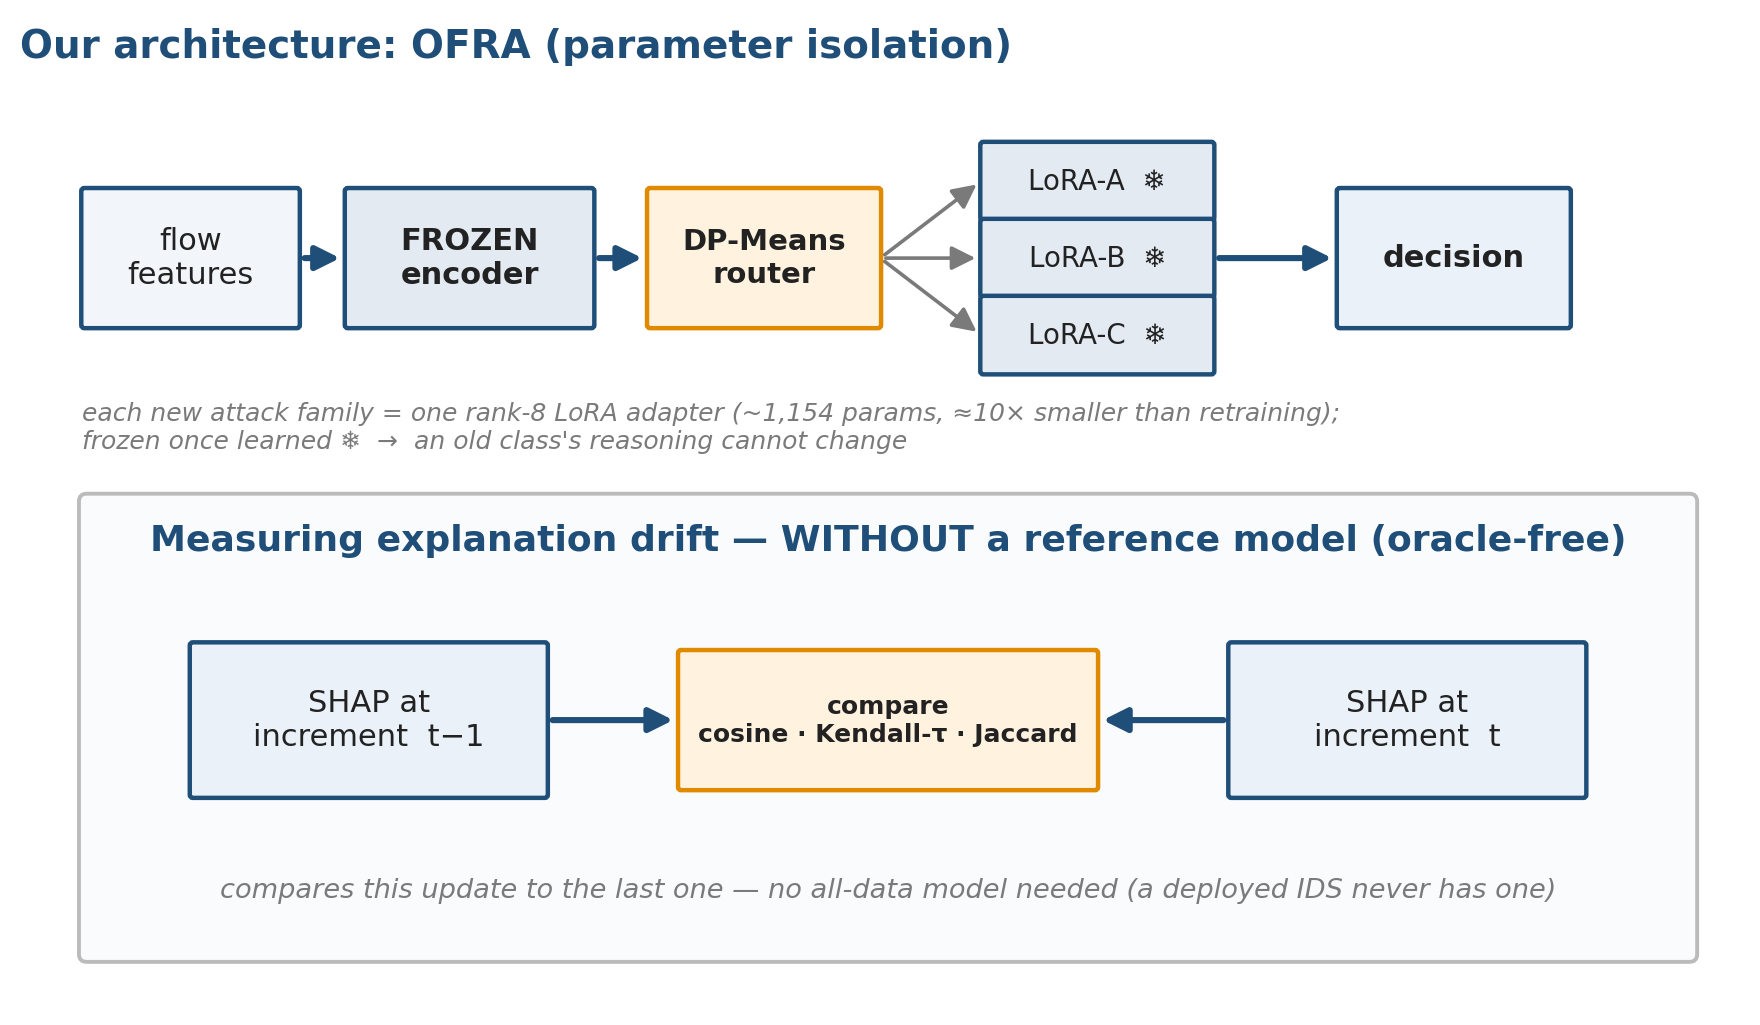
\includegraphics[width=0.92\textwidth]{fig/arch.png}
\caption{OFRA. A frozen shared encoder feeds a per-attack-family rank-$8$
adapter, frozen once learned and selected at inference by an oracle-free
DP-Means router. Drift is measured by comparing attributions at increment $t$
against $t{-}1$, with no all-data reference model.}
\label{fig:arch}
\end{figure*}

OFRA (Fig.~\ref{fig:arch}) has four parts.

\textbf{Frozen shared encoder.} A two-layer MLP ($d\!\to\!128\!\to\!128$) is
trained on the first task and then frozen. Because the representation never
moves, an old family's feature space---and therefore its attribution---cannot
drift as a side effect of later encoder updates.

\textbf{Per-family adapters.} Each new attack family is learned as its own rank-$8$
LoRA adapter~\cite{hu2021lora} on top of the frozen encoder (roughly $1.2$K
trainable parameters), and frozen once learned. Learning a new attack therefore
cannot overwrite an old one along its isolated path.

\textbf{Oracle-free router.} At inference a DP-Means~\cite{kulis2012revisiting}
router selects the family adapter by prototype distance, without a task
identifier---the realistic deployment case.

\textbf{Bounded exemplar memory.} Fifty raw exemplars per family support replay
and calibration.

The design gives a structural property: on the \emph{isolated path}, an old
family's frozen adapter cannot change, so its attribution is invariant by
construction. We stress that this is a property of the isolated path, not a
guarantee about the deployed decision (Section~\ref{sec:results-drift}), and we
do not claim OFRA is the most accurate detector---Section~\ref{sec:results-pareto}
shows it is not.

%% ============================================================
\section{Oracle-Free Silent-Drift Protocol}
\label{sec:protocol}

For every preserved old family at every increment we compute attributions with
SHAP and an input-gradient estimator, rank features, and compare the top-$15$
sets across the two most recent increments by Jaccard, cosine and
Kendall-$\tau$. Two safeguards keep the signal honest. A
\emph{forgetting-versus-data-shift decomposition} separates attribution change
caused by the model from change caused by input distribution shift, so a low
overlap cannot be waved away as a data artefact. A \emph{deletion-based
faithfulness check} confirms that the ranked features are the ones the model
actually uses. The protocol needs only two consecutive deployed checkpoints; it
never constructs the all-data reference model that continuity methods assume.

%% ============================================================
\section{ETG: Explanation-Trust Gate}
\label{sec:etg}

\begin{figure*}[t]
\centering
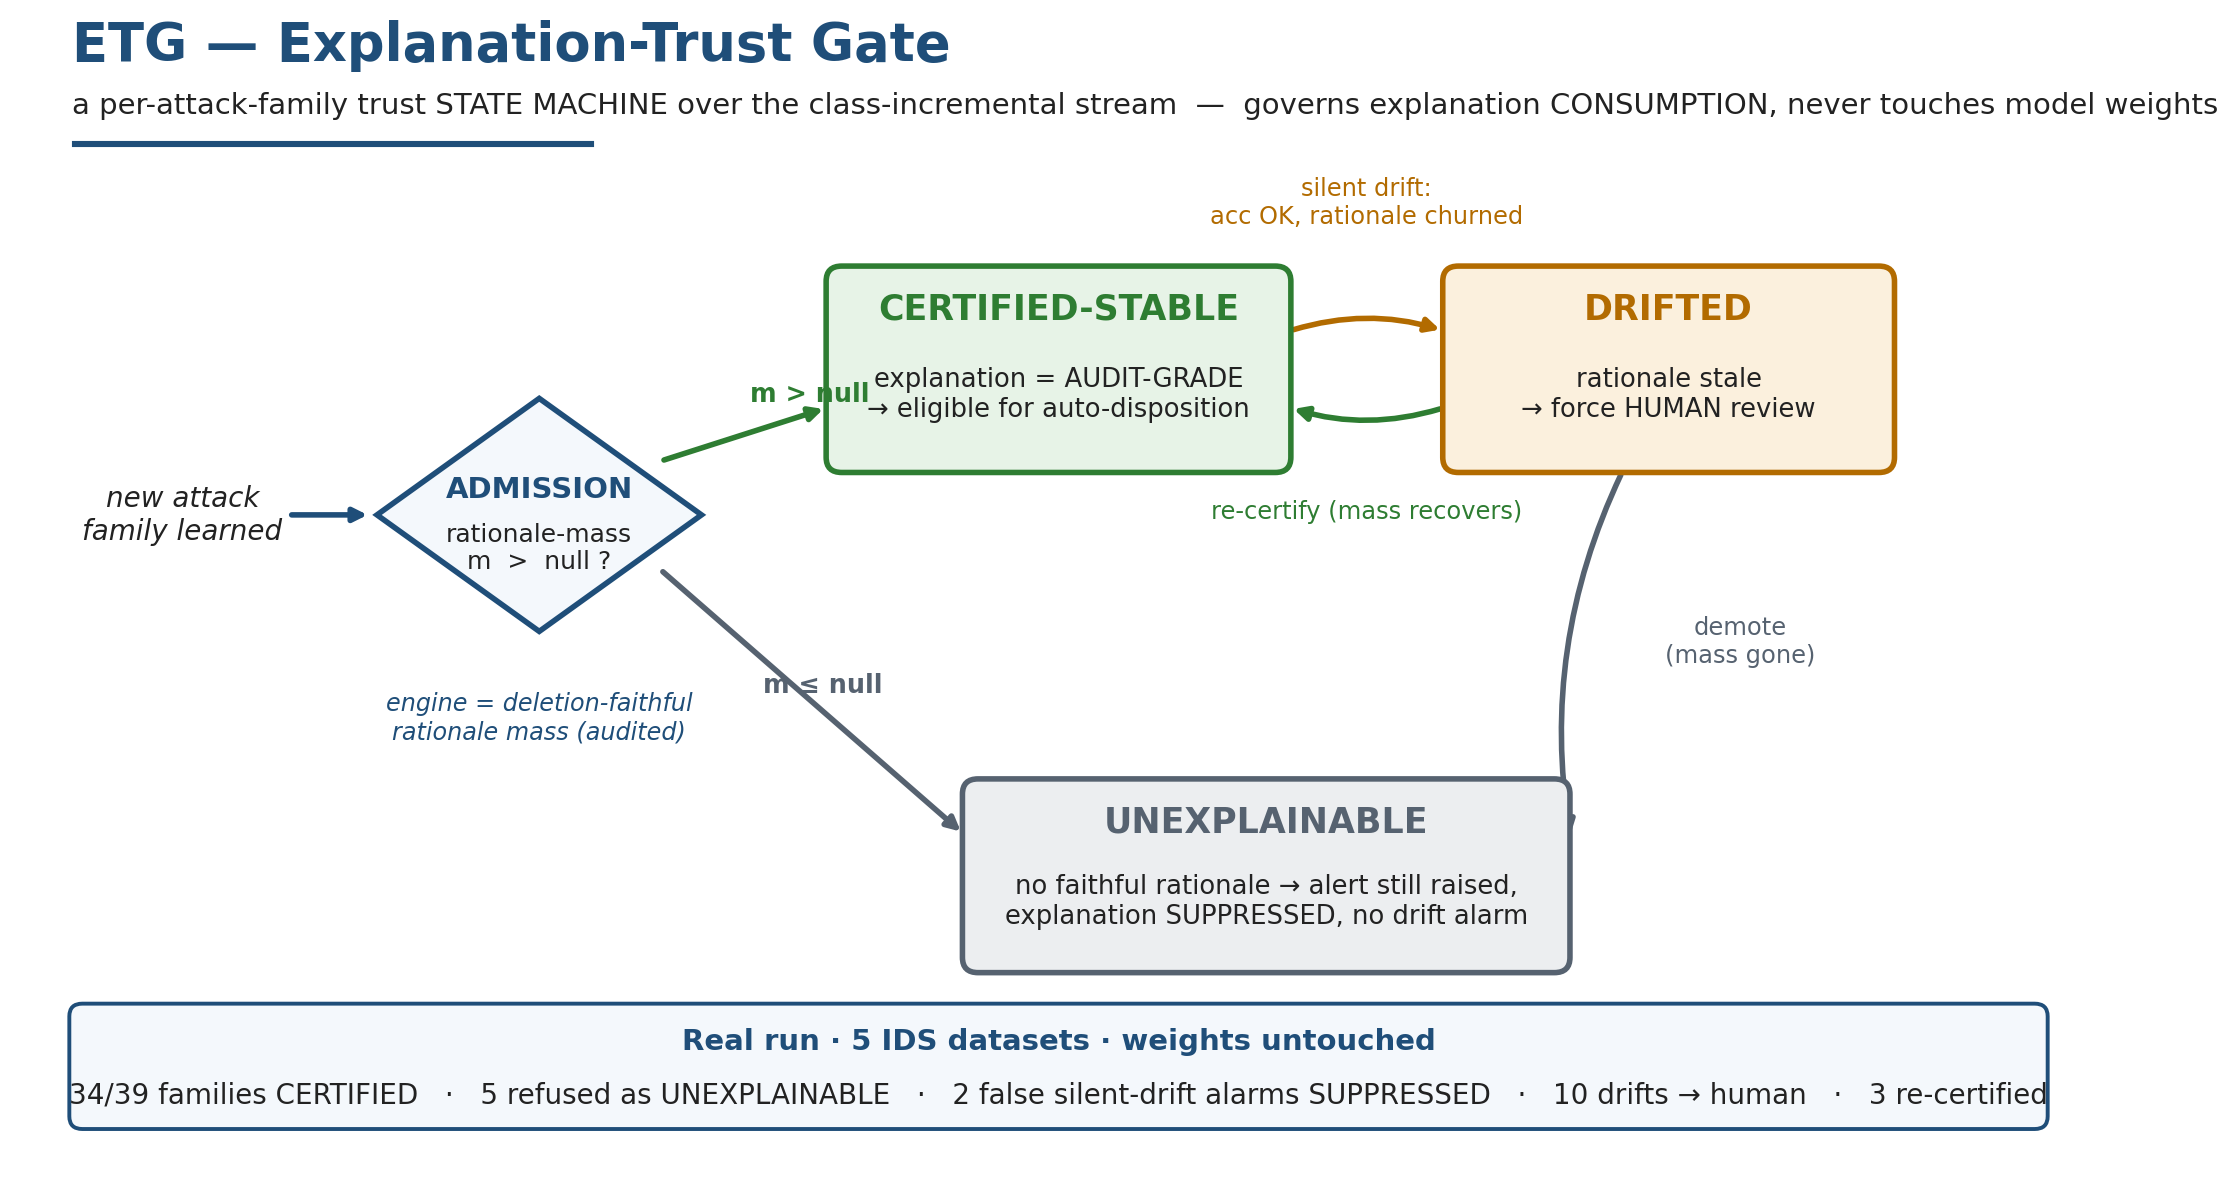
\includegraphics[width=0.98\textwidth]{fig/etg.png}
\caption{ETG state machine. A family is admitted only if a faithful, concentrated
rationale exists (rationale-mass above a random null); certified families are
monitored for drift; ill-posed families are declared unexplainable; drifted
families are routed to a human. ETG never changes model weights.}
\label{fig:etg}
\end{figure*}

OFRA's structural stability covers the isolated path, but not the decision the
router ships (Section~\ref{sec:results-drift}). Rather than try to prevent that
residual drift---which we show is hard to do without paying accuracy
(Section~\ref{sec:results-pareto})---ETG \emph{governs} it. ETG changes no
weights; it governs how much each family's explanation may be trusted.

\subsection{Engine: rationale mass}
Before drift can be tracked, a faithful rationale must exist. For family $c$ we
rank features by occlusion importance (the drop in the class-$c$ softmax
probability when a feature is zeroed) and define its \emph{rationale mass} as the
joint deletion-gap of the top-$15$ occlusion features. A family is admitted only
if its mass exceeds a random-$15$ null (the $95$th percentile of masses from
random feature sets). This metric is reproducible, stable under a split-half
check, near-zero for an anti-rationale (bottom-$15$) baseline, and
random-controlled. Where mass is essentially zero, explanation stability is
ill-posed and a drift alarm there would be noise.

\subsection{State machine}
Each family carries a persistent state (Fig.~\ref{fig:etg}):
\[
\begin{gathered}
\textsf{UNCERTIFIED}\to\{\textsf{CERTIFIED\text{-}STABLE},\\
\textsf{UNEXPLAINABLE}\}\to\textsf{DRIFTED}\\
\to\{\text{re-certify},\,\textsf{UNEXPLAINABLE}\}.
\end{gathered}
\]
On admission, a family whose mass clears the null becomes
\textsf{CERTIFIED-STABLE} and its reference rationale is frozen; otherwise it is
\textsf{UNEXPLAINABLE}. At a later increment, if accuracy is preserved but the
top-$15$ Jaccard against the certified reference falls below $0.70$, the family
becomes \textsf{DRIFTED}. A drifted family whose mass later recovers may return
to \textsf{CERTIFIED-STABLE}; otherwise it is demoted.

\subsection{Action policy}
The states drive operator-facing actions. A \textsf{CERTIFIED-STABLE} explanation
is audit-grade and eligible for auto-disposition. A \textsf{DRIFTED} alert is
force-routed to a human and its stale rationale is withheld. An
\textsf{UNEXPLAINABLE} family still raises its detection alert---detection is
untouched---but its unreliable explanation is suppressed and no drift alarm is
emitted for it. The auto-maintained per-family trust ledger (family, increment,
mass, action) is the artefact a SOC actually consumes.

%% ============================================================
\section{Experimental Setup}
\label{sec:setup}

We use five datasets---NSL-KDD, UNSW-NB15, CIC-IDS-2017, CIC-IDS-2018 and
NF-ToN-IoT-v2---in attack-family-incremental order, each with five seeds. We
compare eight methods spanning the three CL families: a naive lower bound,
EWC~\cite{kirkpatrick2017overcoming}, LwF~\cite{li2017learning},
Replay, DP-Means Replay, iCaRL~\cite{rebuffi2017icarl}, a recent frozen-backbone
baseline (NCM-Frozen), and OFRA. Forgetting is the mean drop of each old family's
accuracy from its first-learned value; significance uses paired tests with
Holm correction over the family of comparisons~\cite{cohen1988statistical,wohlin2012experimentation}.

%% ============================================================
\section{Results}
\label{sec:results}

\subsection{Silent drift: the $0\%$ is isolated-path only}
\label{sec:results-drift}

Accuracy-preserving shared-parameter baselines silently drift $3$--$100\%$
depending on the dataset, with every baseline separated from OFRA at $p<0.001$
and Cohen's $d\approx 6$. On the isolated path OFRA drifts $0\%$ by construction.
This headline is real but partial: the deployed decision is produced \emph{after}
the oracle-free router, which can re-route old-attack inputs as new families are
added. Measuring drift at the decision level (Table~\ref{tab:drift},
Fig.~\ref{fig:bridge}) gives $2.3\%$ pooled over $26$ runs---$6.7\%$ on NSL-KDD
and $6.2\%$ on CIC-IDS-2017, $0\%$ on UNSW-NB15 and CIC-IDS-2018. This residual is
exactly the blind spot ETG governs.

\begin{figure*}[t]
\centering
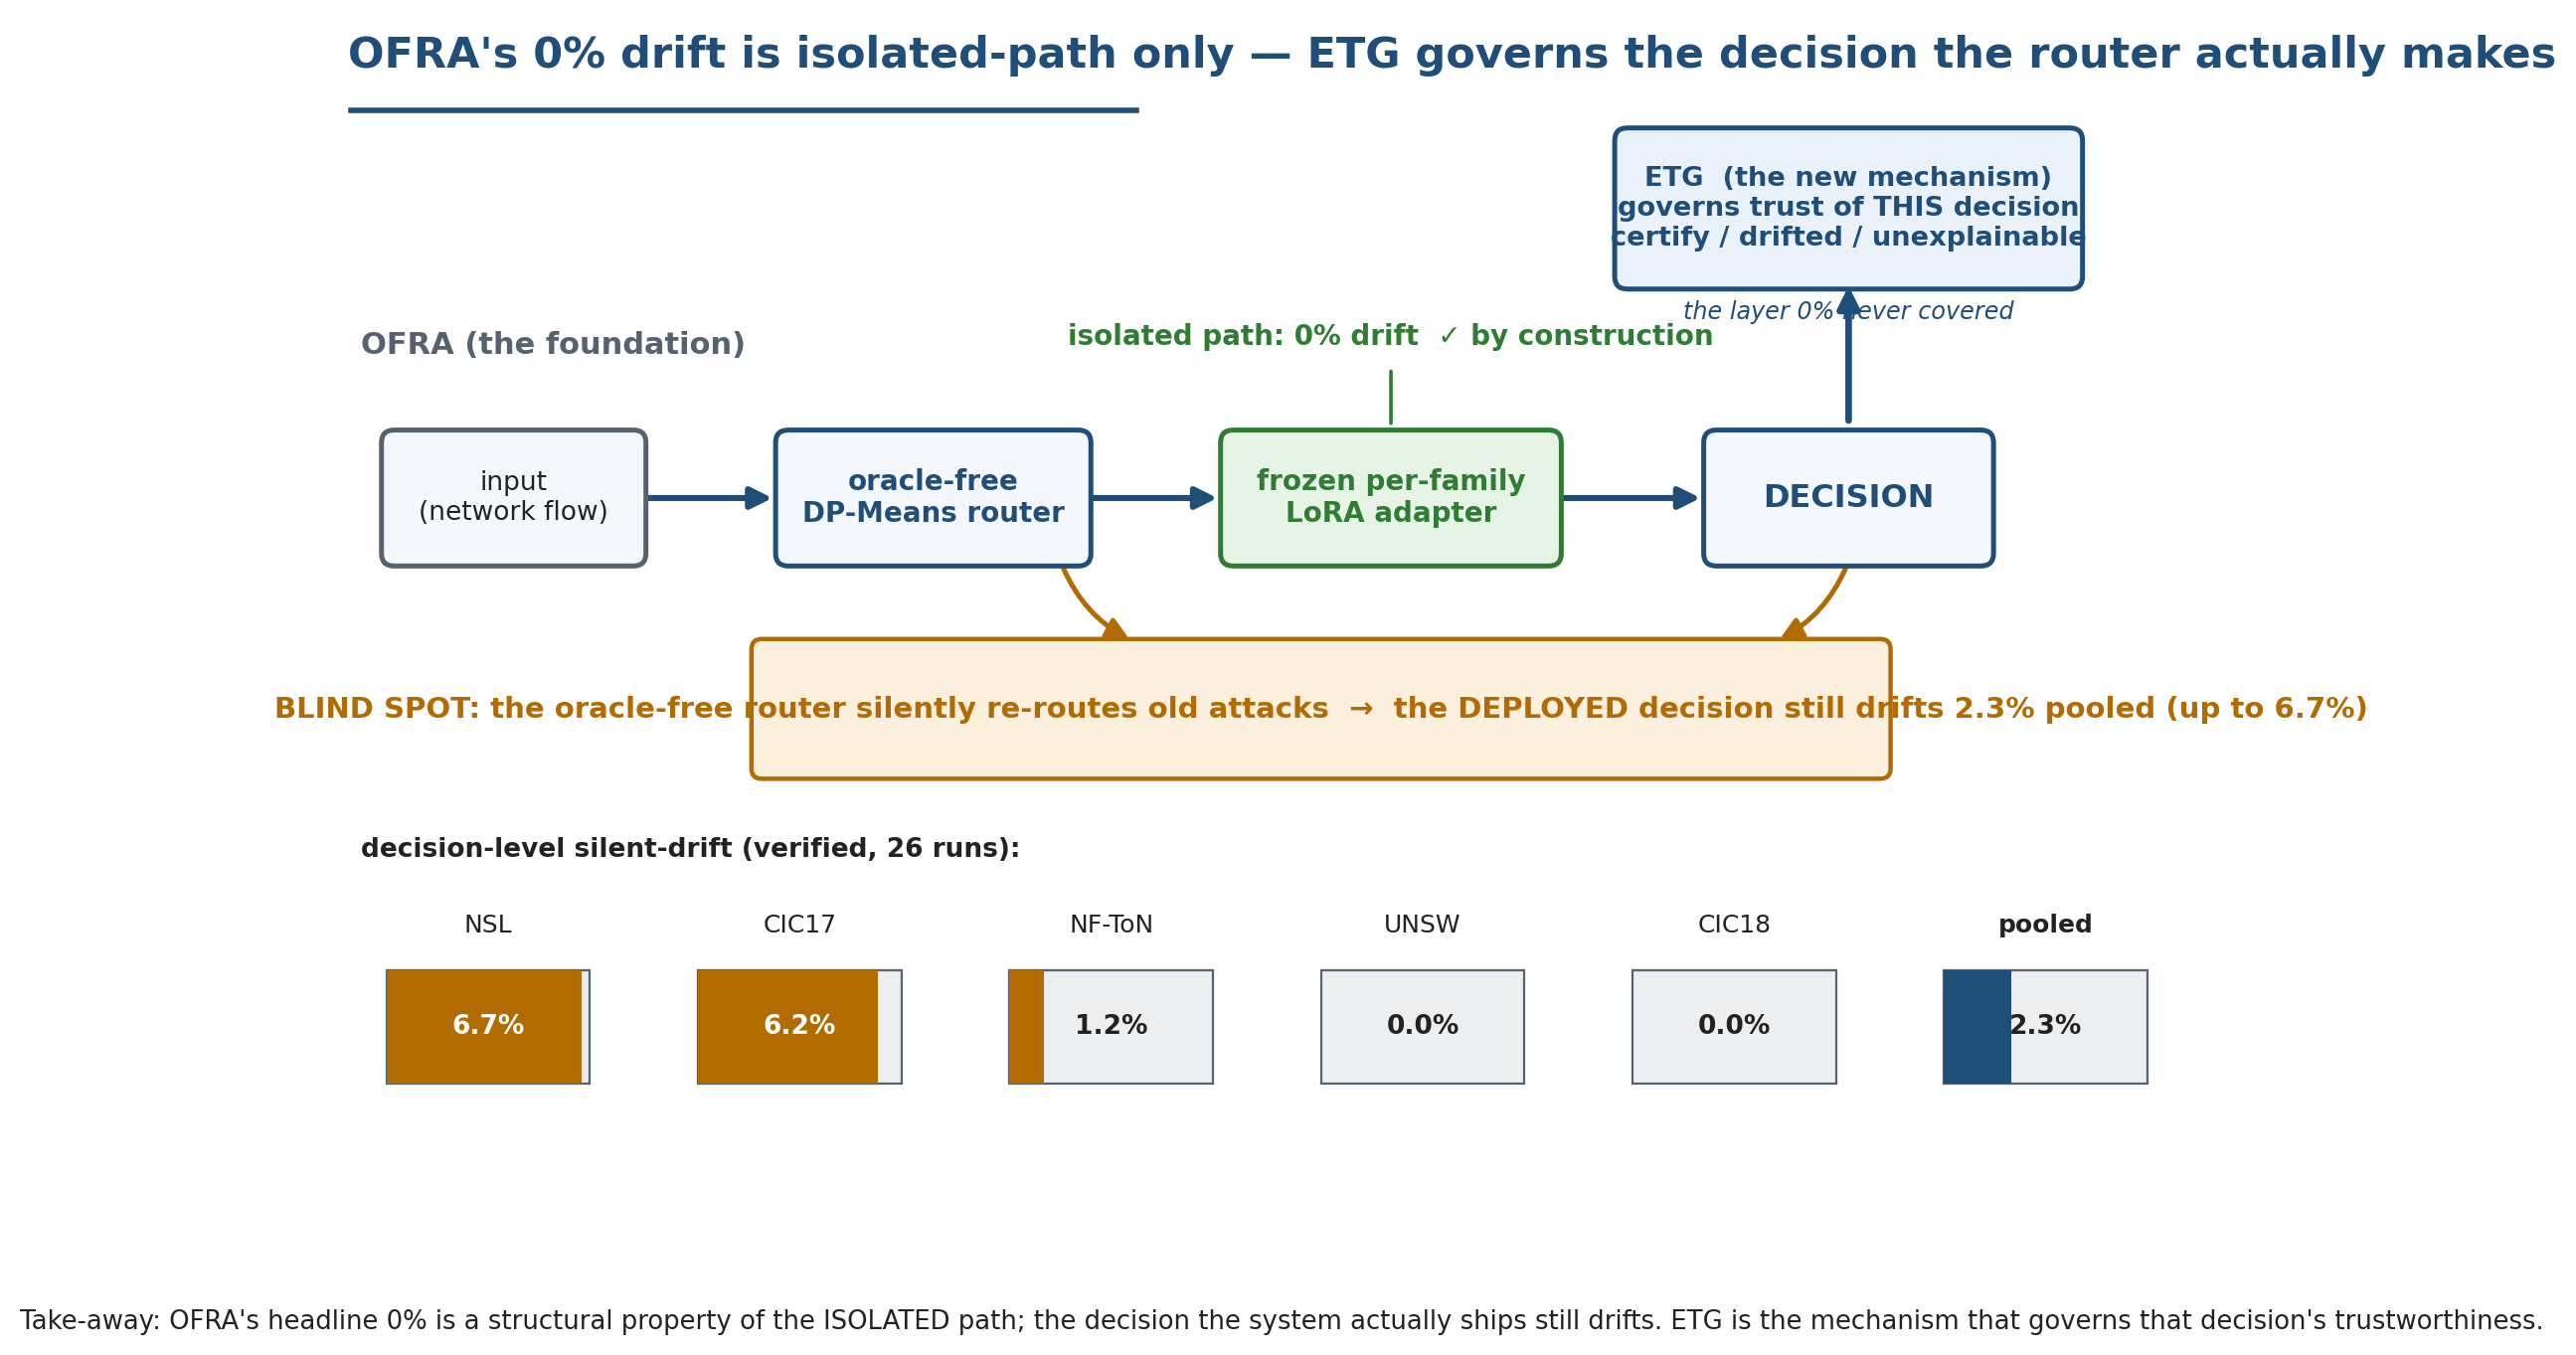
\includegraphics[width=0.9\textwidth]{fig/bridge.png}
\caption{OFRA's $0\%$ is a structural property of the isolated path; after the
oracle-free router the shipped decision still drifts $2.3\%$ pooled (up to
$6.7\%$). ETG governs the trustworthiness of that decision.}
\label{fig:bridge}
\end{figure*}

\begin{table}[t]
\caption{Silent-drift rate (\%). Baselines are shared-parameter models; the OFRA
column is the honest \emph{deployed} (decision-level) drift. OFRA's isolated path
is $0\%$ by construction.}
\label{tab:drift}
\centering
\begin{tabular}{lcccc}
\toprule
Dataset & Naive & Replay & DP-Means & \textbf{OFRA} \\
\midrule
NSL-KDD        & 53 & 15 & 28 & \textbf{6.7} \\
UNSW-NB15      & 61 & 37 & 43 & \textbf{0.0} \\
CIC-IDS-2017   & 79 & 82 & 85 & \textbf{6.2} \\
CIC-IDS-2018   & 100 & 81 & 92 & \textbf{0.0} \\
NF-ToN-IoT-v2  & 17 & 3 & 6 & \textbf{1.2} \\
\midrule
\multicolumn{4}{l}{OFRA pooled (decision-level)} & \textbf{2.3} \\
\bottomrule
\end{tabular}
\end{table}

\subsection{Forgetting and the accuracy trade-off}
\label{sec:results-pareto}

OFRA lowers forgetting by a geometric-mean factor of $3.1\times$ against the
strongest baseline (Table~\ref{tab:forget}), significant on four of five datasets
after Holm correction. We report CIC-IDS-2018's $1.3\times$ as not significant
($p=0.10$) rather than hiding it. This comes at an honest accuracy cost of
$8$--$16$~pp and with roughly an order of magnitude fewer trainable parameters
per family. We do \emph{not} claim state-of-the-art accuracy: OFRA is a different
operating point on the accuracy--stability plane, not an overall winner.

We also asked whether a new training-time mechanism could simply \emph{prevent}
the decision-level drift. Across our five datasets and an eight-angle search over
three custom regularisers, frozen isolation empirically Pareto-dominated every
prevention configuration we tried---it reached $0\%$ isolated-path drift at no
worse accuracy and lower forgetting than any constrained alternative. We treat
this as an empirical observation on our benchmark, not a proof of impossibility;
it is why we chose to \emph{govern} the residual drift rather than fight it.

\begin{table}[t]
\caption{Forgetting reduction of OFRA versus the strongest baseline
(five seeds, Holm-corrected), and OFRA's accuracy cost.}
\label{tab:forget}
\centering\small\setlength{\tabcolsep}{3pt}
\begin{tabular}{lccc}
\toprule
Dataset & Forgetting reduction & $p_{\mathrm{Holm}}$ & Acc.\ cost \\
\midrule
NSL-KDD        & $6.6\times$ & $0.009$   & $-16.0$~pp \\
UNSW-NB15      & $3.5\times$ & $8.4\!\times\!10^{-6}$ & $-7.7$~pp \\
CIC-IDS-2017   & $2.9\times$ & $0.027$   & $-10.6$~pp \\
CIC-IDS-2018   & $1.3\times$ & $0.10$ (n.s.) & $-7.8$~pp \\
NF-ToN-IoT-v2  & $2.3\times$ & ---       & --- \\
\midrule
Geometric mean & $\mathbf{3.1\times}$ & & \\
\bottomrule
\end{tabular}
\end{table}

\subsection{ETG: the trust ledger}
\label{sec:results-etg}

Table~\ref{tab:etg} is the artefact ETG produces. Across the five datasets it
certifies $34$ of $39$ families, refuses five as unexplainable, suppresses two
silent-drift alarms on families with no faithful rationale, and routes ten real
drifts to a human (with three later re-certified). The refusals and suppressions
are work a plain accuracy monitor or drift monitor cannot do: they are the cases
where an alarm would be noise, or where a certificate would be dishonest.

\begin{table}[t]
\caption{ETG per-family trust ledger (five datasets, five seeds). ETG never
changes model weights.}
\label{tab:etg}
\centering\scriptsize\setlength{\tabcolsep}{2pt}
\begin{tabular}{lcccc}
\toprule
Dataset & Certified & Refused & Alarms supp. & Drifts$\to$human \\
\midrule
NSL-KDD        & 5/5  & 0 & 0 & 2 \\
UNSW-NB15      & 9/10 & 1 & 1 & 1 \\
CIC-IDS-2017   & 6/7  & 1 & 0 & 2 \\
CIC-IDS-2018   & 7/7  & 0 & 0 & 4 \\
NF-ToN-IoT-v2  & 7/10 & 3 & 1 & 1 \\
\midrule
\textbf{Total} & \textbf{34/39} & \textbf{5} & \textbf{2} & \textbf{10} \\
\bottomrule
\end{tabular}
\end{table}

\textbf{The engine is load-bearing.} Replacing the deletion-faithful engine with
ordinary input-gradient attribution changes $19$ of $39$ admission decisions
(occlusion admits $34/39$; input-gradient admits $19/39$). The faithfulness of
the attribution is not an implementation detail---it decides half the ledger.

\textbf{Stability across seeds.} The admission partition is stable: NSL-KDD,
CIC-IDS-2018 and NF-ToN-IoT-v2 have zero standard deviation across five seeds,
while UNSW-NB15 ($9.2\pm0.4$) and CIC-IDS-2017 ($6.2\pm0.8$) wobble only on
families whose mass sits near the null.

\textbf{Why govern, not auto-repair.} A natural alternative is to penalise the
model to restore a drifted family's rationale. We implemented a triggered,
family-local, occlusion-anchored repair. Globally it looks almost free---accuracy
barely moves---but a per-family audit shows it silently destroys a rare attack
family: repairing UNSW-NB15 Fuzzers/Reconnaissance drops Shellcode accuracy by
$\sim\!45$~pp, and CIC-IDS-2017 repairs cost Infiltration $\sim\!14$~pp.
Auto-repair is therefore unsafe on this data; ETG routes drift to a human
instead.

%% ============================================================
\section{Discussion}
\label{sec:discussion}

The positioning of this work is narrow on purpose. OFRA is oracle-free, unlike
explanation-continuity methods that assume a known task identifier. ETG carries
\emph{per-family persistent state} over the incremental stream, unlike stateless
per-alert trust triage on a static model, and it is gated by a faithfulness test
so that it declares ``unexplainable'' rather than certifying an ill-posed family.
It is a governance layer on top of the detector, not a drift-prevention
algorithm, and it targets exactly the decision-level residue that frozen
isolation leaves uncovered.

%% ============================================================
\section{Supplemental prediction--retention trade-off}
This later, bounded RQ2 study compares a refreshed benign--attack gate with an attack-family learner. AR removes gate distillation while retaining DER-style family replay and weight alignment; it is distinct from frozen OFRA isolation and from ETG. Tables~\ref{tab:cse-new-seed-tradeoff}--\ref{tab:cse-new-seed-tests} reproduce the lead's rounded CSE18 follow-up computation. AR is not confirmed as a final-accuracy improvement over Replay-BS: lower forgetting costs about 4--5 percentage points of mean incremental BAcc. Non-significance is not equivalence. These new-seed results do not replace the historical OFRA tests, establish an explanation-drift or governance benefit, or close the locked RQ1/RQ3 and substantive-innovation requirements. Full remaining-method reporting and an independent final-result consumer remain pending.
% Complete Section 87 descriptive extension: saved Section 64/74/82 values only.
% Equal-weight seed means and sample SD (n-1); no forward pass or hypothesis tests.
\begin{table*}[t]
\centering\small
\caption{All 45 CSE18 cells: nine methods, seeds 5--9, calibration target 2\%. Descriptive extension: not in the registered decision.}\label{tab:cse-all45-descriptive}
\setlength{\tabcolsep}{4pt}
\begin{tabular}{lrrrrr}
\toprule
Method & Mean inc. BAcc & Final BAcc & Forget (pp) & ADR & Test FPR \\
\midrule
AR & $81.67\pm4.35$ & $77.44\pm2.89$ & $-0.24\pm6.32$ & $95.04\pm0.18$ & $1.97\pm0.07$ \\
AA-CIL & $84.73\pm0.56$ & $77.36\pm2.52$ & $4.08\pm3.96$ & $95.04\pm0.18$ & $1.97\pm0.07$ \\
Replay-BS & $86.21\pm0.48$ & $77.52\pm3.84$ & $8.26\pm5.50$ & $94.26\pm1.63$ & $1.99\pm0.06$ \\
Freq & $69.86\pm6.07$ & $61.46\pm17.08$ & $14.25\pm10.11$ & $75.81\pm25.60$ & $2.00\pm0.03$ \\
WACB & $65.54\pm11.16$ & $50.12\pm26.27$ & $19.93\pm16.55$ & $50.75\pm44.77$ & $2.03\pm0.04$ \\
KD+WA & $78.94\pm4.62$ & $70.44\pm2.33$ & $3.31\pm4.25$ & $95.23\pm0.41$ & $1.95\pm0.06$ \\
Replay & $55.94\pm3.44$ & $21.37\pm5.40$ & $40.88\pm5.21$ & $7.06\pm10.95$ & $2.04\pm0.03$ \\
DER++ & $53.21\pm5.35$ & $19.70\pm10.62$ & $36.36\pm19.41$ & $13.37\pm26.88$ & $2.05\pm0.03$ \\
AKD & $72.53\pm9.67$ & $56.73\pm23.43$ & $10.02\pm19.15$ & $74.99\pm35.32$ & $2.00\pm0.03$ \\
\midrule
\multicolumn{6}{l}{Final BAcc by seed (percent; all five values, no selected seeds)} \\
Method & Seed 5 & Seed 6 & Seed 7 & Seed 8 & Seed 9 \\
\midrule
AR & 76.27 & 80.88 & 78.81 & 78.05 & 73.19 \\
AA-CIL & 76.58 & 74.35 & 78.99 & 80.75 & 76.14 \\
Replay-BS & 71.49 & 81.94 & 79.16 & 77.97 & 77.03 \\
Freq & 31.89 & 61.72 & 73.32 & 70.45 & 69.92 \\
WACB & 21.35 & 21.81 & 64.33 & 74.00 & 69.10 \\
KD+WA & 71.82 & 72.67 & 71.49 & 66.89 & 69.35 \\
Replay & 15.13 & 21.23 & 21.41 & 29.92 & 19.16 \\
DER++ & 14.86 & 15.08 & 38.69 & 15.61 & 14.29 \\
AKD & 65.71 & 17.86 & 75.06 & 52.47 & 72.57 \\
\bottomrule
\end{tabular}
\par\smallskip\begin{minipage}{.97\textwidth}\footnotesize
Upper panel: equal-weight means $\pm$ sample SD across five seeds, not confidence intervals. Values are percentages except signed forgetting in percentage points, including Normal; negative values are not clipped. The 2\% target is a calibration setting, not a guaranteed test FPR. Source: published Section 64 single-seed releases (AR, AA-CIL, Replay-BS, Freq, WACB), Section 74 descriptive releases (KD+WA, Replay, DER++), and Section 82 descriptive releases (AKD). Aggregation uses saved scalar metrics only; AKD ADR/FPR aliases are checked against the saved final operating point. No training, inference, confusion-matrix recomputation, or new significance test is involved. The 40 original cells and five separately appended AKD cells are counted once; Replay-LA is not an additional physical method. This nine-method extension is not in the registered decision: the original five-method decision and its failures remain unchanged, and the four additional methods are descriptive only. These are new seeds on the same exposed CSE dataset, not independent-dataset confirmation. Complete-seed interim releases do not authorize tuning, early stopping, or reselection.
\end{minipage}
\end{table*}

% Presentation of the lead's rounded recomputation in work-order Sections 71--72.
% No training, inference, or independent statistical recomputation by this table.
\begin{table*}[t]
\centering\small
\caption{CSE18, paired seeds 5--9 ($n=5$): retention--plasticity trade-off. Blind seeds 5--9; externals evaluated from saved checkpoints, no retraining (1\% panel).}\label{tab:cse-new-seed-tradeoff}
\begin{tabular}{llrrrrr}
\toprule
Target & Method & Mean inc. BAcc & Final BAcc & Forget (pp) & ADR & Test FPR \\
\midrule
2\% & AR & 81.7 & 77.4 & $-0.2$ & 95.0 & 1.97 \\
 & AA-CIL & 84.7 & 77.4 & 4.1 & 95.0 & 1.97 \\
 & Replay-BS & 86.2 & 77.5 & 8.3 & 94.3 & 1.99 \\
 & Freq & 69.9 & 61.5 & 14.2 & 75.8 & 2.00 \\
 & WACB & 65.5 & 50.1 & 19.9 & 50.7 & 2.03 \\
\midrule
1\% & AR & 80.9 & 76.3 & $-0.8$ & 94.5 & 1.00 \\
 & AA-CIL & 83.7 & 76.2 & 3.8 & 94.5 & 1.00 \\
 & Replay-BS & 84.7 & 74.4 & 8.2 & 93.3 & 1.01 \\
 & Freq & 63.9 & 58.3 & 11.4 & 68.2 & 1.00 \\
 & WACB & 50.2 & 28.7 & 15.8 & 18.8 & 1.03 \\
\bottomrule
\end{tabular}
\par\smallskip\begin{minipage}{.97\textwidth}\footnotesize
Values are percentages except signed forgetting in percentage points; negative forgetting is retained, not clipped. Rounded means are transcribed from the lead's recomputation recorded in work-order Sections 71--72, except the completed 2\% ADR and test-FPR columns, which are arithmetic means of the five saved final values per method in the published Section 64 seed releases. No confusion matrices or statistical tests were recomputed for this completion. The 2\% panel derives from the 25 published decision cells; the 1\% panel combines saved AR/AA/BS operating points with Freq/WACB checkpoint evaluation. No model was retrained for the 1\% panel. ``Blind seeds'' describes the initially withheld seed results, not an independent dataset: the design followed unsealing of the earlier CSE round, uses the same exposed dataset, and complete single-seed interim releases preceded this final summary. No early stopping, tuning, or criterion changes followed those releases.
\end{minipage}
\end{table*}

\begin{table*}[t]
\centering\small
\caption{CSE18 lead-reported paired tests at 1\% ($n=5$). Differences are AR minus reference, in percentage points.}\label{tab:cse-new-seed-tests}
\begin{tabular}{llrrr}
\toprule
Reference & Endpoint (alternative) & Difference & One-sided $t$ $p$ & Exact sign-flip $p$ \\
\midrule
Freq & Final BAcc ($>$) & 18.0 & .045 & .031 \\
Freq & Mean inc. BAcc ($>$) & 17.0 & .005 & .031 \\
WACB & Final BAcc ($>$) & 47.6 & .001 & .031 \\
WACB & Mean inc. BAcc ($>$) & 30.7 & .003 & .031 \\
Replay-BS & Final BAcc ($>$) & 1.9 & .059 & .062 \\
\bottomrule
\end{tabular}
\par\smallskip\begin{minipage}{.97\textwidth}\footnotesize
Rounded values from work-order Sections 71--72; paired $t$ has four degrees of freedom, and sign-flip enumerates all 32 sign assignments. These are reported tests, not new tests executed during typesetting. At 1\%, the lead reports AR forgetting differences of $-12.1$pp versus Freq and $-16.5$pp versus WACB; harm is not significant against the lowest-forgetting external (Freq). Thus the external half of H-low passes for AR, but the Replay-BS superiority half fails, so the conjunction is not confirmed. This is not an equivalence finding. At 2\%, the registered final-BAcc superiority criterion also fails (AR minus BS $-0.08\pm3.11$pp; reported one-sided $p\geq.52$), while the other three criteria pass. No new round or selection is implied. AR has the lowest mean forgetting among these five available decision methods, not among unreported variants.
\end{minipage}
\end{table*}


\section{Limitations}
\label{sec:limits}

We state the boundaries plainly. ETG governs explanation \emph{consumption}; it
does not improve detection accuracy, and its value assumes explanations are
actually used and must be trustworthy. Its cost is not zero: drifted and
unexplainable families are routed to humans, a coverage/analyst-load cost that
should be measured over a live stream. Rationale mass is computed on class-mean
probes; per-sample governance is future work. The evidence for ETG is at
proof-of-concept maturity---a small number of alarms per dataset---and we
deliberately do \emph{not} claim that a drift alarm localises which feature the
model migrated to, because that reliance-migration interpretation did not survive
a random-controlled test; a \textsf{DRIFTED} verdict is only a conservative
``stop auto-trusting'' signal. Finally, a sixth dataset (CIC-IoT-2023) is not yet
included.

%% ============================================================
\section{Conclusion}
\label{sec:conclusion}

We treated explanation stability as a measurable property of class-incremental
intrusion detection. An oracle-free protocol makes silent explanation drift
visible without an all-data reference model; OFRA is an oracle-free detector
whose isolated paths are stable by construction, offered as a Pareto operating
point rather than an accuracy winner; and ETG governs the trustworthiness of the
deployed decision that OFRA's structural $0\%$ does not cover, certifying
families whose rationale is faithful, refusing those whose rationale is ill-posed,
and routing drift to a human rather than silently retraining. Future work will
formalise the certificate and its thresholds, lift certification from the isolated
path to the routed decision, and evaluate alarm latency and false-alarm rate on a
streaming deployment.

The later AR follow-up reinforces the need to report operating points rather
than an overall winner. The lead's CSE18 summary places final BAcc at 77.4\%
for AR and 77.5\% for Replay-BS at the 2\% target, with lower AR forgetting but
about 4--5 pp lower mean incremental BAcc. At 1\%, AR exceeds Freq and WACB,
yet the 1.9 pp advantage over Replay-BS is not significant, so H-low remains
unconfirmed. No equivalence, causal gate explanation, or new method-selection
success follows. These tests are distinct from the historical OFRA
CIC-IDS-2018 result ($p=0.10$, not significant), and neither changes it.
The published follow-up tables identify the lead's rounded recomputation;
independent final statistical consumption and remaining-method descriptive
reporting are still pending. The study's predictive trade-off does not by
itself complete RQ1/RQ3 or the substantive-innovation gate.

\par\vspace{5pt}\noindent\textit{Code, results, and the source of this paper are
available at} \url{https://github.com/1838904818/Class-IL}.

%% ============================================================
\bibliographystyle{IEEEtran}
\bibliography{references}

\end{document}
